\documentclass[aspectratio=169]{beamer}

\usepackage{listings}
\usepackage[utf8,latin1]{inputenc}
\usepackage[style = apa, backend = biber, natbib = true]{biblatex}
\addbibresource{../../literature/lit.bib}

\makeatletter \def\newblock{\beamer@newblock} \makeatother

\beamertemplatenavigationsymbolsempty
\setbeamertemplate{itemize items}[circle]
\setbeamertemplate{section in toc}[circle]
\mode<beamer>{\setbeamercolor{math text displayed}{fg=iwmgray}}
\setbeamercolor{block body}{bg=iwmorange!50!white}
\setbeamercolor{block title}{fg=white, bg=iwmorange}

% Definitions for biblatex
\setbeamercolor{bibliography entry note}{fg=iwmgray}
\setbeamercolor{bibliography entry author}{fg=iwmgray}
\setbeamertemplate{bibliography item}{}

\definecolor{iwmorange}{RGB}{255,105,0}
\definecolor{iwmgray}{RGB}{67,79,79}
\definecolor{iwmblue}{RGB}{60,180,220}
\definecolor{iwmgreen}{RGB}{145,200,110}
\definecolor{iwmpurple}{RGB}{120,0,75}

\setbeamercolor{title}{fg=iwmorange}
\setbeamercolor{frametitle}{fg=iwmorange}
\setbeamercolor{structure}{fg=iwmorange}
\setbeamercolor{normal text}{fg=iwmgray}
\setbeamercolor{author}{fg=iwmgray}
\setbeamercolor{date}{fg=iwmgray}

\lstset{language = R,%
  basicstyle = \ttfamily\color{iwmgray},
  frame = single,
  rulecolor = \color{iwmgray},
  commentstyle = \slshape\color{iwmgreen},
  keywordstyle = \bfseries\color{iwmgray},
  identifierstyle = \color{iwmpurple},
  stringstyle = \color{iwmblue},
  numbers = none,%left,numberstyle = \tiny,
  basewidth = {.5em, .4em},
  showstringspaces = false,
  emphstyle = \color{red!50!white}}

\title{Generalized linear mixed-effects models}
\author{Nora Wickelmaier}
\date{Last modified: \today}

\AtBeginSection[]{
  \frame{
    \tableofcontents[sectionstyle=show/hide, subsectionstyle=show/show/hide]}}

% \setbeamertemplate{headline}{
%  \begin{beamercolorbox}{section in head}
%    \vskip5pt\insertsectionnavigationhorizontal{\paperwidth}{}{}\vskip2pt
%  \end{beamercolorbox}
% }

\setbeamertemplate{footline}{\vskip-2pt\hfill\insertframenumber$\;$\vskip2pt}

\begin{document}

\begin{frame}{}
\thispagestyle{empty}
\titlepage
\end{frame}

% \begin{frame}{Outline}
% \tableofcontents
% \end{frame}

\begin{frame}[fragile]{GLMMs}
  \begin{itemize}
    \item Like linear models, mixed-effects models can be extended so that they
      allow for response variables that have arbitrary distributions
    \item A GLM(M) is a specific combination of a response distribution, a link
      function, and a linear predictor 
    \item We can choose (almost) all the link functions that work with
      \texttt{glm()} for \texttt{glmer()}
  \end{itemize}
\begin{lstlisting}
## Family name       Link functions
   binomial          logit, probit, log, cloglog
   gaussian          identity, log, inverse
   Gamma             identity, inverse, log
   inverse.gaussian  1/mu^2, identity, inverse, log
   poisson           log, identity, sqrt
\end{lstlisting}
\end{frame}

\begin{frame}{Example: 1989 Bangladesh Fertility Survey\footnote{Reanalysis of https://repsychling.github.io/SMLP2024/glmm.html}}
Subset containing variables about
  \begin{itemize}
    \item District where women live
    \item Age (mean centered)
    \item Living children (coded 1~=~no~children, 2~=~one~child,
      3~=~two~children, 4~=~three or more children)
    \item Use of artificial contraception (yes or no)
    \item Area where women live is rural or urban
  \end{itemize}
\end{frame}

\begin{frame}{}
  \begin{block}{Exercise}
    \begin{itemize}
      \item Read the data into R
      \item Create a plot showing the probability to use artificial
        contraception depending on age
      \item Draw separate lines for number of living children
      \item Make two panels: one for rural and one for urban
      \item Use \texttt{ggplot2} or \texttt{lattice}\\[1.8ex]
            Hint: Use \texttt{geom\_smooth()} for \texttt{ggplot2} and
            \texttt{type = "smooth"} for \texttt{lattice::xyplot()}
    \end{itemize}
  \end{block}
\end{frame}

\begin{frame}[fragile]{Data set contra}
\begin{lstlisting}
dat <- read.table("data/contra.dat", header = TRUE)

dat$districtID <- factor(dat$districtID)
dat$childCode <- factor(dat$childCode,
                        levels = 1:4,
                        labels = c("0", "1", "2", "3+"))
dat$isUrban <- factor(dat$isUrban,
                      levels = 0:1,
                      labels = c("n", "y"))

# simplify names
names(dat) <- c("dist", "use", "livch", "age", "urban")
\end{lstlisting}
\end{frame}

\begin{frame}{Visualization}
  \centering
  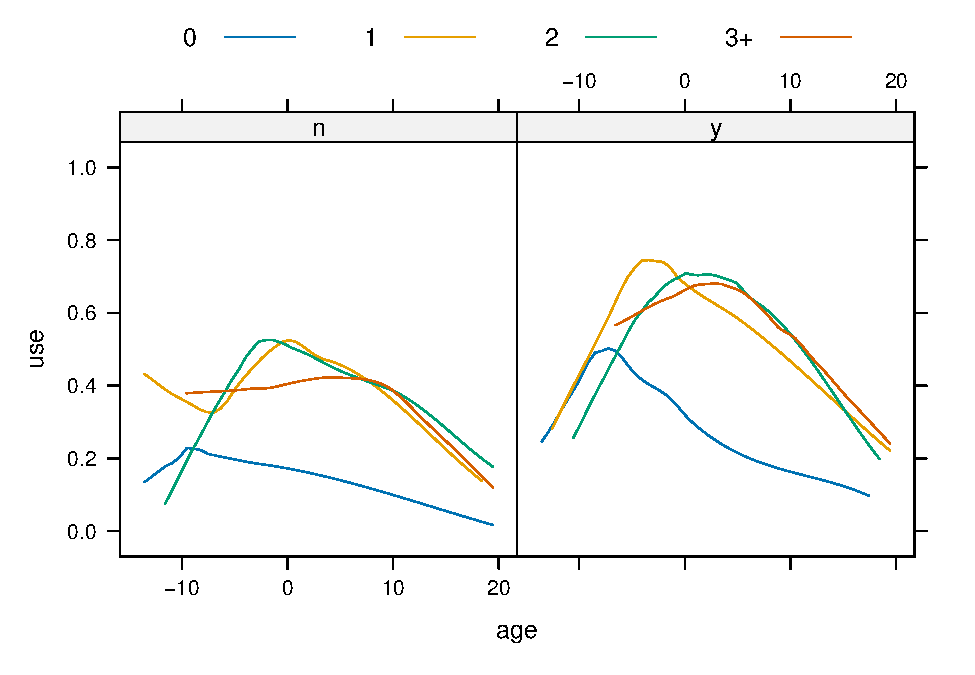
\includegraphics[scale = .7]{../figures/contra_data}
\end{frame}

\begin{frame}{GLMM}
  \begin{itemize}
    \item Fit the following model to the data
      \[
        log(\frac{p}{1-p}) = \beta_0 + \beta_1 age + \beta_2 age^2 + \beta_3
        urban + \beta_4 livch + \upsilon_0
      \]
      with $\upsilon_0 \sim N(0, \sigma_{\upsilon_0}^2)$
    \item We are assuming that there are differences between the districts, so
      we add a random intercept for district
    \item What are your conclusions about differences between women with and
      without children?
  \end{itemize}
\end{frame}

\begin{frame}{Dichotomize \texttt{livch}}
  \begin{itemize}
    \item We create a new factor \texttt{children} that indicates if a woman has
      children or not (independently of how many)
    \item Next, we add an interaction term for \texttt{children} and
      \texttt{age} to our model
      \[
        log(\frac{p}{1-p}) = \beta_0 + \beta_1 age + \beta_2 children + \beta_3
        (age \times children) + \beta_4 age^2 + \beta_5 urban + \upsilon_0
      \]
      with $\upsilon_0 \sim N(0, \sigma_{\upsilon_0}^2)$
    \item How can we compare which model fits the data better?
  \end{itemize}
\end{frame}

\begin{frame}[fragile]{Nested random effect}
  \begin{itemize}
    \item It turns out that districts are very big and can incorporate rural as
      well as urban areas
    \item The districts can be very different depending on this
    \item Add a random intercept to the model taking this into account
\begin{lstlisting}
xtabs( ~ urban + dist, dat)
xtabs( ~ urban + factor(urban:dist), dat)
xtabs( ~ dist + factor(dist:urban), dat) |> print(zero = ".")
\end{lstlisting}
    \item Compare the models -- what is your conclusion?
    \item What exactly is the difference between these models?
  \end{itemize}
\end{frame}

\begin{frame}[fragile]{Model predictions}
\begin{lstlisting}
# Compare models
data.frame(models = c("gm1", "gm2", "gm3"),
           df = AIC(gm1, gm2, gm3)[, 1],
           AIC = AIC(gm1, gm2, gm3)[, 2],
           BIC = BIC(gm1, gm2, gm3)[, 2],
           deviance = c(deviance(gm1), deviance(gm2), deviance(gm3)))

# Model predictions
newdat <- data.frame(children = factor(rep(c("true", "false"),
                                       each = 2)),
                     urban = factor(rep(c("y", "n"), times = 2)),
                     age = 0)
newdat$pre <- predict(gm3, type = "response", newdata = newdat,
                      re.form = NA)
\end{lstlisting}
\end{frame}

\begin{frame}{}
  \begin{block}{Exercise}
    \begin{itemize}
      \item Create a new data frame with variables \texttt{children} ("true",
        "false"), \texttt{urban} ("yes", "no"), and \texttt{age} (ranging from
        $-14$ to 20)
      \item Add a prediction for each combination of the three variables
      \item Draw a plot of your predictions
      \item Interpret the results
    \end{itemize}
  \end{block}
\end{frame}

\begin{frame}{Summary}
  \begin{itemize}
    \item From the data plot we can see a quadratic trend in the probability by
      age.
    \item The patterns for women with children are similar and we do not need to
      distinguish between 1, 2, and 3+ children.
    \item We do distinguish between those women who do not have children and
      those with children. This shows up in a significant $age \times children$
      interaction term.
  \end{itemize}
\end{frame}

%\appendix
%%\begin{frame}[allowframebreaks]{References}
%\begin{frame}{References}
%  \printbibliography
%\end{frame}

\end{document}

